\documentclass[12pt]{scrartcl}
\usepackage[sexy]{james}
\usepackage[noend]{algpseudocode}
\setlength{\marginparwidth}{2cm}
\usepackage{answers}
\usepackage{array}
\usepackage{tikz}
\usepackage{graphicx}
\newenvironment{allintypewriter}{\ttfamily}{\par}
\usepackage{listings}
\usepackage{xcolor}
\usetikzlibrary{arrows.meta}
\usepackage{color}
\usepackage{mathtools}
\newcommand{\U}{\mathcal{U}}
\newcommand{\E}{\mathbb{E}}
\usetikzlibrary{arrows}
\Newassociation{hint}{hintitem}{all-hints}
\renewcommand{\solutionextension}{out}
\renewenvironment{hintitem}[1]{\item[\bfseries #1.]}{}
\renewcommand{\O}{\mathcal{O}}
\declaretheorem[style=thmbluebox,name={Chinese Remainder Theorem}]{CRT}
\renewcommand{\theCRT}{\Alph{CRT}}
\setlength\parindent{0pt}
\usepackage{sansmath}
\usepackage{pgfplots}

\usetikzlibrary{automata}
\usetikzlibrary{positioning}  %                 ...positioning nodes
\usetikzlibrary{arrows}       %                 ...customizing arrows
\newcommand{\eqdef}{=\vcentcolon}
\newcommand{\tr}{{\rm tr\ }}
\newcommand{\im}{{\rm Im\ }}
\newcommand{\spann}{{\rm span\ }}
\newcommand{\Col}{{\rm Col\ }}
\newcommand{\Row}{{\rm Row\ }}
\newcommand{\dint}{\displaystyle\int}
\newcommand{\dt}{\ {\rm d }t}
\newcommand{\PP}{\mathbb{P}}
\newcommand{\horizontal}{\par\noindent\rule{\textwidth}{0.4pt}}
\usepackage[top=3cm,left=3cm,right=3cm,bottom=3cm]{geometry}
\newcommand{\mref}[3][red]{\hypersetup{linkcolor=#1}\cref{#2}{#3}\hypersetup{linkcolor=blue}}%<<<changed

\tikzset{node distance=4.5cm, % Minimum distance between two nodes. Change if necessary.
         every state/.style={ % Sets the properties for each state
           semithick,
           fill=cyan!40},
         initial text={},     % No label on start arrow
         double distance=4pt, % Adjust appearance of accept states
         every edge/.style={  % Sets the properties for each transition
         draw,
           ->,>=stealth',     % Makes edges directed with bold arrowheads
           auto,
           semithick}}


% Start of document.
\newcommand{\sep}{\hspace*{.5em}}

\pgfplotsset{compat=1.18}
\begin{document}
\title{MATH410: Homework 6}
\author{James Zhang\thanks{Email: \mailto{jzhang72@terpmail.umd.edu}}}
\date{\today}

\definecolor{dkgreen}{rgb}{0,0.6,0}
\definecolor{gray}{rgb}{0.5,0.5,0.5}
\definecolor{mauve}{rgb}{0.58,0,0.82}

\lstset{frame=tb,
  language=Java,
  aboveskip=3mm,
  belowskip=3mm,
  showstringspaces=false,
  columns=flexible,
  basicstyle={\small\ttfamily},
  numbers=left,
  numberstyle=\tiny\color{gray},
  keywordstyle=\color{blue},
  commentstyle=\color{dkgreen},
  stringstyle=\color{mauve},
  breaklines=true,
  breakatwhitespace=true,
  tabsize=3
}

\maketitle

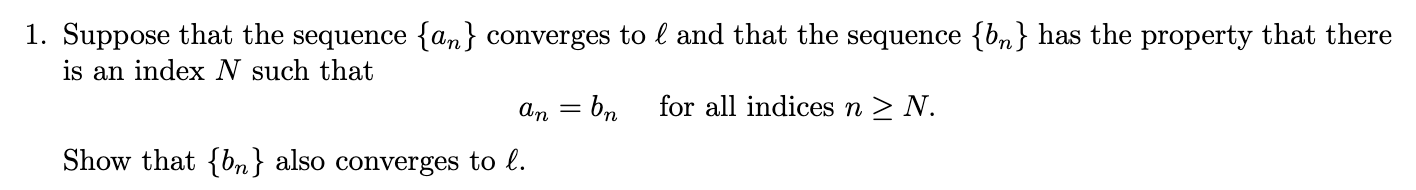
\includegraphics[width=14cm]{1.png}

\begin{proof}
  
\hfill

Let $f(x) = x^5 + 5x + 1$. Note that $f$ is continuous and differentiable because 
it is a polynomial. Note that $f(-1) = -3 < 0$ and $f(0) = 1 > 0$. Note that 
$0 \in (-3, 1)$. By the IVT, $\exists \ c \in (-1, 0)$ such that $f(c) = 0$.
Now I will show that this $c$ is unique. Assume on the contrary that there are two solutions, 
such that $f(a) = 0 = f(b)$. By Rolle's Theorem, 
$\exists \ z \in (a,b)$ such that $f'(z) = 0$ but note that 
\[f'(x) = 5x^4 + 5\]
and so \[f'(z) = 5z^4 + 5 = 0 \implies z^4 = -1\]
and so $z$ is not a real number, which is a contradiction. Therefore, the solution 
$c$ is unique.

\end{proof}

\newpage

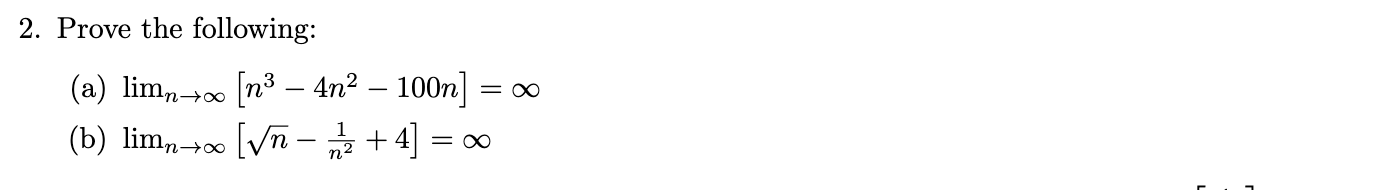
\includegraphics[width=14cm]{2.png}

\begin{proof}
  
\hfill

First note that the inverse $h^{-1}$ exists by a theorem because 
$h$ is strictly monotone, so it is 1-1 and therefore has an inverse. 
Further note that $f$ and $h$ are differentiable on $\RR$ and so we can 
apply the Chain Rule to find 
\[g'(x) = f'(h^{-1}(x)) \cdot (h^{-1})'(x)\]
Now recall that $h'(x) > 0 \ \forall \ x$, and so we can use the corollary in class which states that 
\[(h^{-1})'(x) = \frac{1}{h'(h^{-1}(x))}\]
By substitution, 
\[g'(x) = \frac{f'(h^{-1}(x))}{h'(h^{-1}(x))}\]

\end{proof}

\newpage 

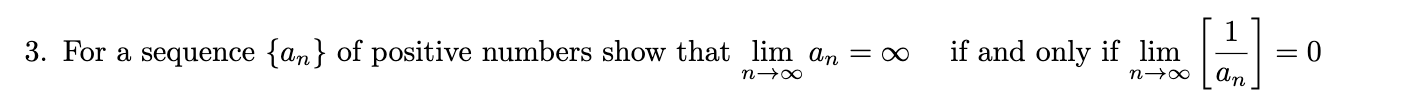
\includegraphics[width=14cm]{3.png}

\begin{proof}
  
\hfill

We WTS that $\exists \ c \in \RR$ s.t. $f(x) = cg(x)$. 
Note that in order for the above equation to hold for all $x$, then if $g(x) \neq 0$, then 
both $f(x) \neq 0 \ \forall \ x$ and $g'(x) \neq x \ \forall \ x$, too.
Let $h: \RR \to \RR$ be $h(x) = \frac{f(x)}{g(x)}$. Therefore, it is sufficient now 
to show that $h(x) = c \ \forall \ x$, or in other words, we wish to show that 
$h$ is constant.
Note that $h$ is differentiable 
because $f$ and $g$ are. By the Identity Criterion, $h$ is constant if and only if $h'(x) = 0 \ \forall \ x$. 
Let us compute $h'(x)$.
\[h'(x) = \frac{f'(x)g(x) - g'(x)f(x)}{(g'(x))^2}\]
by the quotient rule. Note that the numerator is $0$ for all $x$, which is a given and that 
$g'(x) \neq 0 \ \forall \ x$. Therefore, 
\[h'(x) = 0 \ \forall \ x \implies h(x) = c \ \forall \ x\]
by the Identity Criterion, and so we equivalently $f(x) = cg(x) \ \forall \ x$. 

\end{proof}

\newpage 

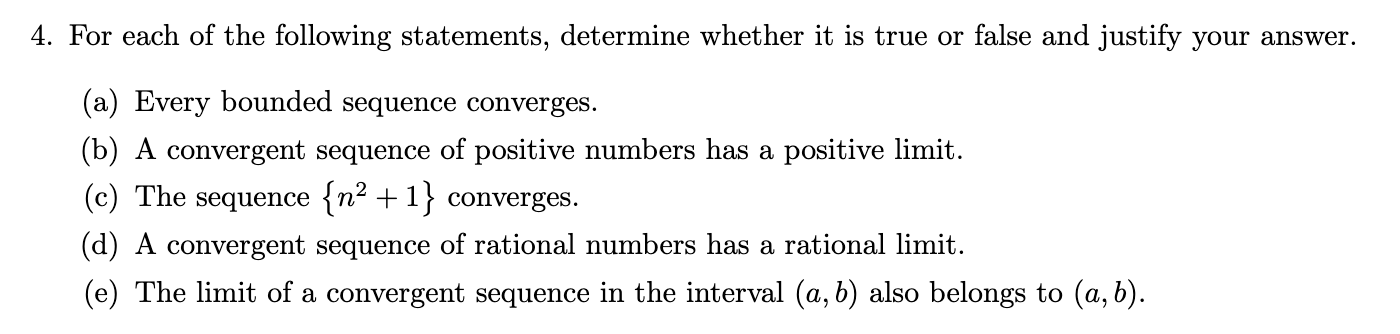
\includegraphics[width=14cm]{4.png}

\begin{proof}
  
\hfill

Recall the Identity Criterion (Differ by a Constant) which states that given some interval 
$I$ and functions $g: I \to \RR$ and $h: I \to \RR$, $f$ and $g$ differ by a constant 
if and only if $g'(x) = h'(x) \ \forall \ x$. Note that $D$ is not an interval. Let 
us define $g: D \to \RR$ and $h: D \to \RR$ such that  
\[g(x) = \begin{cases}
  x + 2, \ x > 0\\
  x - 1, \ x < 0
\end{cases} \text{ and  } h(x) = x \ \forall \ \in D\]

Note that $g'(x) = 1 = h'(x) \ \forall \ x \in D$. However, it is clear that $g$ and $h$ 
do not differ by a constant. $g(-1) = -2$ and $h(-1) = -1$ but 
$g(2) = 4$ and $h(1) = 1$. Thus, we have found a counterexample, and so the functions 
$g$ and $h$ do not necessarily differ by a constant, as desired.

\end{proof}

\newpage 

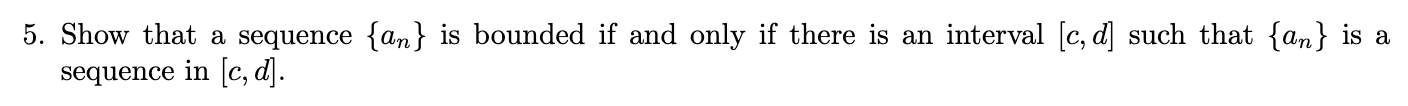
\includegraphics[width=14cm]{5.png}

\begin{proof}
  
\hfill

Let us create a function $h: \RR \to \RR$ such that $h(x) = |f(x)|^2 + |g(x)|^2 \ \forall \ x$. 
Note that $h$ is differentiable because $f$ and $g$ are. Now 
note that $|f(x)|^2 = f(x)$ and $|g(x)|^2 = g(x)^2 \ \forall x$. Therefore, 
$h(x) = f(x)^2 + g(x)^2$. By the Identity Criterion, $h$ is 
constant if and only if $h'(x) = 0 \ \forall \ x$. Let us compute $h'(x)$. 
\[h'(x) = 2f(x) f'(x) + 2g(x) g'(x) \ \forall \ x\]
by the Chain Rule twice. Let us show that this derivative is $0$.
Recall that $f'(x) = g(x)$ and $g'(x) = -f(x) \ \forall \ x$ by the given. 
Note that $g(x)$ and $f'(x)$ are the same sign for all $x$, and 
$f(x)$ and $f'(x)$ are different signs for all $x$. 
\[\frac{g(x)}{f'(x)} = \frac{-f(x)}{g'(x)} = 1 \ \forall \ x\]
Therefore, by cross multiplying the above,
\[g(x)g'(x) = -f(x)f'(x) \implies g(x)g'(x) + f(x)f'(x) = 0\]
Multiplying the above by $2$ we obtain $h'(x)$
\[h'(x) = 2g(x)g'(x) + 2f(x)f'(x) = 0 \ \forall \ x\]
Therefore, $h'(x) = 0 \ \forall \ x$ and so by the Identity Criterion, $h(x)$ is a constant 
for all $x$. Specifically, $h(x) = 1 \ \forall \ x$ because 
at $x=0$, 
\[h(x) = |f(0)|^2 + |g(x)|^2 = 0 + 1 = 1\]
Therefore, $h(x) = 1 \ \forall \ x$ as desired. 


\end{proof}

\newpage


\includegraphics[width=14cm]{6.png}

\begin{proof}
  
\hfill

Let $u, v \in [a,b]$ such that $u < v$. Note that $f$ and $g$ satisfy the conditions of the Cauchy Mean Value Theorem, 
which gives us that 
\[\exists \ c \in (u, v) \text{ s.t. } \frac{f'(c)}{g'(c)} = \frac{f(u) - f(v)}{g(u) - g(v)}\]
Equivalently, we can wrap both sides of the equation in absolute value and the equality still holds
\[\frac{|f'(c)|}{|g'(c)|} = \frac{|f(u) - f(v)|}{|g(u) - g(v)|}\]
\[|f(u) - f(v)| = \frac{|f'(c)|}{|g'(c)|} |g(u) - g(v)|\]
Note that $|f'(x)| \geq |g'(x)| > 0 \ \forall \ x \implies \frac{|f'(x)|}{|g'(x)|} \geq 1 \ \forall \ x$. Therefore, 
\[|f(u) - f(v)| \geq |g(u) - g(v)| \ \forall \ u, v \in [a,b]\] 
as desired.

\end{proof}

\newpage

\includegraphics[width=14cm]{7.png}

\begin{proof}
  
\hfill

First let us define two auxiliary functions $f: [a,b] \to \RR$ and $g: [a,b] \to \RR$ such that 
$g(x) = \frac{f(x)}{x}$ and $h(x) = \frac{1}{x} \ \forall \ x$. Note that both $f, g$ are continuous 
on $[a,b]$ and differentiable on $(a,b)$ because $f$ is, and we are told that $0 < a < b$. Therefore, 
the conditions for the Cauchy Mean Value Theorem are satisfied, and so 
\[\exists \ c \in (a,b) \text{ s.t. } \frac{g'(c)}{h'(c)} = \frac{g(b) - g(a)}{h(b) - h(a)}\]
Observe that $g'(x) = \frac{xf'(x) - f(x)}{x^2}$ by the quotient rule and $g'(x) = -\frac{1}{x^2}$ by the 
power rule. Substituting known values, we get 
\[\frac{\frac{1}{c^2} (cf'(c) - f(c))}{-\frac{1}{c^2}} = \frac{\frac{f(b)}{b} - \frac{f(a)}{a}}{\frac{1}{b} - \frac{1}{a}}\]
\[f(c) - c'f(c) = \frac{\frac{1}{ab} (af(b) - bf(a))}{\frac{1}{ab}(a-b)}\]
\[f(c) - cf'(c) = \frac{af(b) - bf(a)}{a - b}\]
as desired.

\end{proof}

\newpage
\end{document}

